\documentclass[../main.tex]{subfile}

\begin{document}

\topictitle{Matrices}

A graph can be represented by an adjacency matrix, and a weighted graph can be represented by a distance matrix.

\sectitle{Adjacency matrices}

Each entry in an adjacency matrix describes the number of edges joining the corresponding nodes.

\begin{figure}[H]
\hspace{0.02\linewidth}
\begin{minipage}{0.48\linewidth}
	\centering
	{\renewcommand{\arraystretch}{1.15}
	\begin{tabular}{c|c c c c c c}
		& A & B & C & D & E & F\\
		\hline
		A & 0 & 1 & 0 & 0 & 0 & 0\\
		B & 1 & 0 & 1 & 0 & 2 & 1\\
		C & 0 & 1 & 0 & 1 & 1 & 0\\
		D & 0 & 0 & 1 & 0 & 0 & 1\\
		E & 0 & 2 & 1 & 0 & 0 & 1\\
		F & 0 & 1 & 0 & 1 & 1 & 2
	\end{tabular}}
\end{minipage}\hfill
\begin{minipage}{0.45\linewidth}
	\vspace{2em}
	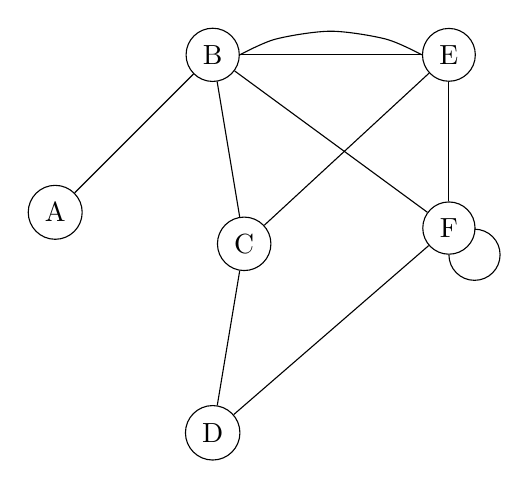
\begin{tikzpicture}
		\node[draw, circle] (A) at (0, 0) {A};
		\node[draw, circle] (B) at (2, 2) {B};
		\node[draw, circle] (C) at (2.4, -0.4) {C};
		\node[draw, circle] (D) at (2, -2.8) {D};
		\node[draw, circle] (E) at (5, 2) {E};
		\node[draw, circle] (F) at (5, -0.2) {F};

		\draw (A) -- (B);
		\draw (B) -- (C);
		\draw (B) -- (E);
		\draw plot[smooth, tension=0.5] coordinates { (B.east) (2.8, 2.2) (3.5, 2.3) (4.2, 2.2) (E.west) };
		\draw (B) -- (F);
		\draw (C) -- (D);
		\draw (C) -- (E);
		\draw (D) -- (F);
		\draw (E) -- (F);
		\draw (F.south) arc (180:450:0.325);
	\end{tikzpicture}
\end{minipage}
\hspace{0.02\linewidth}
\end{figure}

\sectitle{Distance matrices}

Each entry in a distance matrix describes the weight of the edge joining the corresponding nodes, if any.

\begin{figure}[H]
\hspace{0.02\linewidth}
\begin{minipage}{0.48\linewidth}
	\centering
	{\renewcommand{\arraystretch}{1.15}
	\begin{tabular}{c|c c c c c c}
		& A & B & C & D & E \\
		\hline
		A & \--- & 17 & 18 & \--- & \---\\
		B & 17 & \--- & 15 & 19 & 23\\
		C & 18 & 15 & \--- & 20 & \---\\
		D & \--- & 19 & 20 & \--- & 16\\
		E & \--- & 23 & \--- & 16 & \---\\
	\end{tabular}}
\end{minipage}\hfill
\begin{minipage}{0.45\linewidth}
	\vspace{2em}
	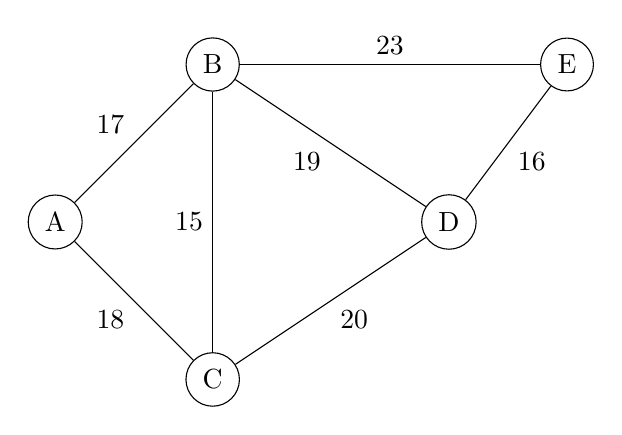
\begin{tikzpicture}
		\node[draw, circle] (A) at (0, 0) {A};
		\node[draw, circle] (B) at (2, 2) {B};
		\node[draw, circle] (C) at (2, -2) {C};
		\node[draw, circle] (D) at (5, 0) {D};
		\node[draw, circle] (E) at (6.5, 2) {E};

		\draw (A) -- node[above left] {17} (B);
		\draw (A) -- node[below left] {18} (C);
		\draw (B) -- node[left] {15} (C);
		\draw (B) -- node[below left] {19} (D);
		\draw (B) -- node[above] {23} (E);
		\draw (C) -- node[below right] {20} (D);
		\draw (D) -- node[below right] {16} (E);
	\end{tikzpicture}
\end{minipage}
\hspace{0.02\linewidth}
\end{figure}

\end{document}
